This subsystem communicates and controls database and Graphical user interface. This is needed
for setting up the initial database for all the users, admin, students, etc.

\subsection{Layer Operating System}
Windows 10

\subsection{Layer Software Dependencies}
Python pyqt4 module 

\subsection{Queue GUI subsystem}
This subsystem will talk with the control subsystem and displays the list of the names of students
in the GUI. This system has two, two-way interfaces. The first is directly connected to the computer recieving
keyboard and mouse input and relaying to the screen. The second passes and receives from Control.

\begin{figure}[h!]
	\centering
 	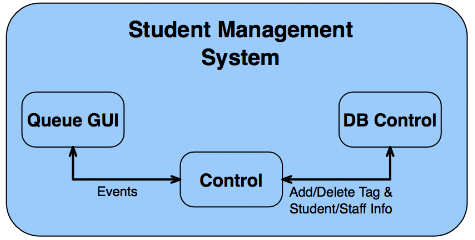
\includegraphics[width=0.60\textwidth]{images/ads_3}
 \caption{Student Management Subsystem}
\end{figure}


\subsubsection{Subsystem Programming Languages}
Python subsystem programming language

\subsection{DB Control subsystem}
This subsystem handles all the data related to students needing to be dismissed by staff. This is the
subsystem that handles forwarding and receiving information from the database. This system has two, two-way interfaces. The first is connected to the database, sending queries and receiving responses. The second passes and receives from Control.


\subsubsection{Subsystem Programming Languages}
Mysql subsystem programming language




